\documentclass{scrartcl}
\usepackage[utf8]{inputenc}
\usepackage{pgf-pie} 
\usepackage{subfigure}
\usepackage{hyperref}
\usepackage{cite}
\usepackage{amsmath}
\usepackage{amssymb}
\usepackage{graphicx}
\documentclass{book}
\renewcommand\thesubsection{\Alph{subsection}}


%opening
\title{Assignment 2}
\author{Daan Spijkers, s1011382\\ Tomás Catalán López, s1081589\\ Willem Lambooy, s1009584}

\begin{document}
\maketitle

\textbf{Note: you can find the GitHub repository at}
\url{github.com/dspijkers/nacu}.

\section{Exercise 1}
\subsection{}
The code for this is in the notebook Assignment2\_1. After running it we get that the fitness of particles $x_1$, $x_2$ and $x_3$ is 730.35, 807.91 and 829.01

\subsection{}
In figure \ref{fig:my_label} we can see how much each point has moved. For more detail, look into the notebook.

\begin{figure}[h!]
    \centering
    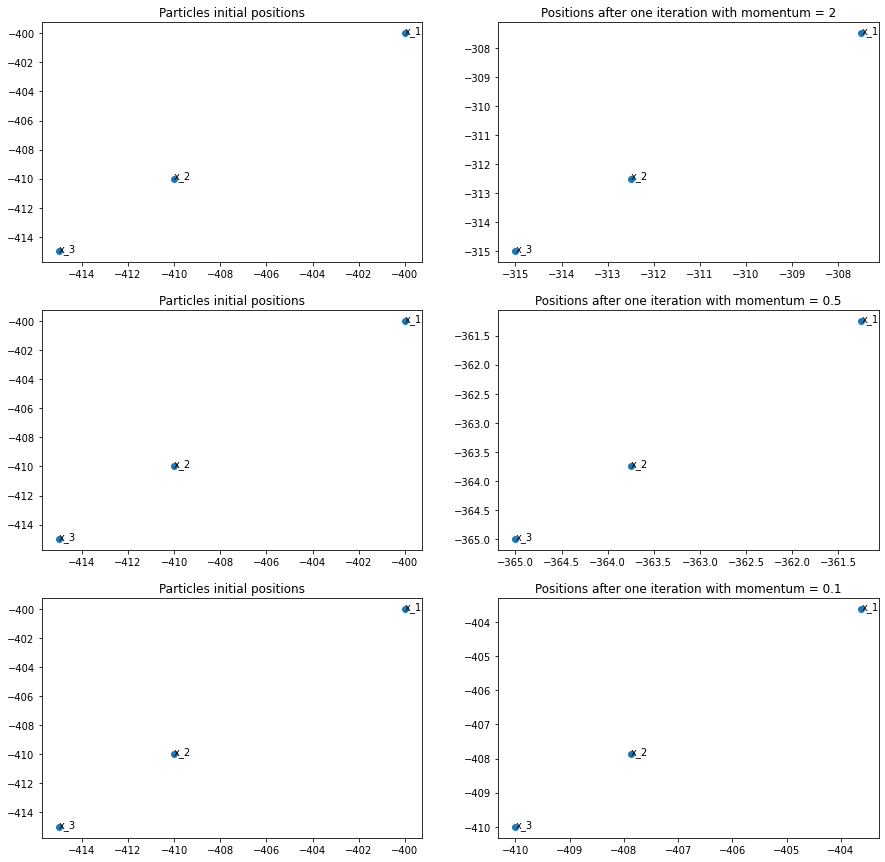
\includegraphics[width=0.65\textwidth]{images/1.png}
    \caption{Scatterplot of $x_1$, $x_2$ and $x_3$ after 1 iteration}
    \label{fig:1l}
\end{figure}

\subsection{}
The momentum has the function to "tune" the position of the particles. If it's $<1$, the best particle will be decreasing its velocity while it's approaxing a better position. If it's $>1$, the particle will be accelerating constantly.

\subsection{}
If we have a higher w, the particles will be moving faster, so it'd be easier to find the optimum if it's far away from the initial position, but it'll be hard to adjust it perfectly in a few iterations, so the computation will take longer.
On the other hand if we have a low momentum the particles would be able to adjust well to the optimum, but they may stop before reaching it (We can see this in Exercise 2.c).

\section{Exercise 2}

\end{document}
